\subsection*{Определение}

\Def Куча — структура данных, которая позволяет добавлять в себя
элементы и получать/извлекать минимум за логарифмическое время.

\Def Бинарная куча  — это такое бинарное дерево, для которого выполнены следующие три условия:
\begin{enumerate}
    \item Значение в любой вершине не больше (если куча для минимума), чем значения её потомков.
    \item На \(i\)-ом слое \(2^i\) вершин, кроме последнего.
    \item Последний слой заполнен слева направо.
\end{enumerate}

\subsection*{Поддержка свойства пирамиды}

\subsubsection*{Реализация кучи на массиве}

Удобнее всего двоичную кучу хранить в виде массива $tree[0..n-1]$, у которого нулевой элемент, $tree[0]$ — элемент в корне, а потомками элемента $tree[i]$ являются $tree[2i+1]$ и $tree[2i+2]$.

\begin{figure}[h!]
        \centering
        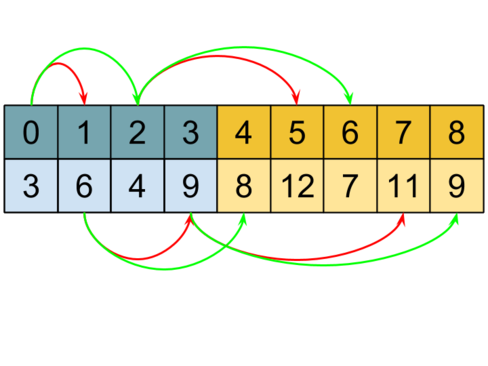
\includegraphics[scale=0.45]{pix/heap_on_an_array.png}
        \caption {Красная стрелка - левый сын, зеленая - правый сын}
        \label{fig:first}
\end{figure}

\subsubsection*{SiftDown}

\Def Просеивание элемента вниз — процедура, погружающая элемент
как можно ниже, пока не выполняется свойство кучи.

\begin{lstlisting}
void Heap::SiftDown(int i) {
  while (2 * i + 1 < size) {
    leftChildIndex = 2 * i + 1;
    rightChildIndex = 2 * i + 2;
    minIndex = i;

    if (tree[leftChildIndex] < tree[minIndex]) {
      minIndex = leftChildIndex;
    }
      
    if (rightChildIndex < size && tree[rightChildIndex] < tree[minIndex]) {
      minIndex = rightChildIndex;
    }

    if (minIndex == i) break;

    swap(tree[i], tree[minIndex]);
    i = minIndex;
  }
}
\end{lstlisting}

\Correctness SiftDown:

Пусть в дереве выполняются все неравенства между детьми и родителями, кроме, может быть, одного элемента $tree_i$, для которого $tree_i$ > $tree_{2i + 1}$ и (или) $tree_i$ > $tree_{2i+2}$. Тогда после выполнения операции SiftDown корректность восстановится.

\drawsome{pix/heap_sift_down.png}

Рассмотрим 5 случаев взаимного соотношения элементов $tree_{i}$ ,$tree_{2i+1}$, $tree_{2i+2}$.
\begin{itemize}
    \item $tree_{i} \leq tree_{2i + 1}$ и $tree_{i} \leq tree_{2i+2}$. Тогда мы заходим в цикл, но ни в первое, ни во второе условие не попадаем, minIndex остается равным i, и мы выходим из функции. Дерево корректно.

    \item $tree_{i}$ > $tree_{2i + 1}$ и $tree_{i} \leq tree_{2i+2}$. Тогда мы заходим в цикл, а после в первое условие. minIndex = leftChildIndex. Во второе условие мы не заходим, в третье тоже. Меняем местами левого ребенка и родителя. Тогда новый родитель больше обоих детей. Тут все корректно. Т.к. оба поддерева изначально были корректны, то мы могли что-то нарушить только в левом поддереве. Идем туда.
     \item $tree_{i} \leq tree_{2i + 1}$ и $tree_{i}$ > $tree_{2i+2}$. Рассуждения аналогичны расссуждению в п.2.
     \item $tree_{i}$ > $tree_{2i + 1}$ и $tree_{i}$ > $tree_{2i+2}$. Тут мы заходим в цикл, а после сразу попадаем в первое условие. minIndex = leftChildIndex.
     Если правый ребенок меньше левого, то он будет новым родителем, т.к. в этом случае правый ребенок является минимальным элементном из трех. Иначе - левый ребенок минимальный. И он станет новым родителем. Меняем родителя с минимальным из детей и идем дальше, нужно проверить, не нарушили  ли мы что-то в ветке, в которой был минимальный ребенок.
    
    \item Если детей нет, в цикл не заходим, все корректно, функция завершает работу. Если есть только один ребенок, то сравнение происходит только с ним. \Endproof
\end{itemize} 

\subsubsection*{SiftUp}

\Def Просеивание элемента вверх — процедура, поднимающая элемент
как можно выше, пока не выполняется свойство кучи.

\begin{lstlisting}
void Heap::SiftUp(int i) {
  int parentIndex = (i - 1) / 2;
  while (i > 0 && tree[i] < tree[parentIndex]) {
    swap(tree[i], tree[parentIndex]);
    i = parentIndex;
    parentIndex = (i - 1) / 2;
  }
}
\end{lstlisting}

\Correctness SiftUp:

Пусть в дереве выполняются все неравенства между детьми и родителями, кроме, может быть, одного элемента $tree_i$, для которого  $tree_i$ < $tree_{(i-1)/2}$ Тогда после выполнения операции SiftUp корректность восстановится.

\drawsome{pix/heap_sift_up.png}

Рассмотрим 2 случая:
\begin{itemize}
    \item Если элемент корневой или $tree_{i} \geq tree_{(i-1)/2}$ тогда дерево корректно, и в цикл мы не заходим, функция завершает выполнение.
    \item Если $tree_{i}$ < $tree_{(i-1)/2}$, то меняем местами родителя и ребенка. Новый родитель не увеличивается, поэтому неравенства между новым родителем и другим ребенком остаются корректными, при этом восстанавливаются неравенства между родителем и двумя детьми. В поддеревьях все ок. Но могло что-то нарушиться выше, поэтому текущий родитель становится ребенком, и процесс повторяется. \Endproof
\end{itemize} 

Выполняя операции SiftUp() и SiftDown() мы переходим между уровнями, на каждом из которых выполняем C = const количество операций. Высота дерева - $log(n)$, поэтому каждая из операций выполняется за время, не превосходящее $C \cdot log(n)$. Таким образом асимптотика $O(log(n))$.

\pagebreak